\documentclass[tikz,border=10pt]{standalone}
\usetikzlibrary{calc}
% scale: 0.02 units per pixel, origin at O (pixel 224.4, 222.0), y flipped
\begin{document}
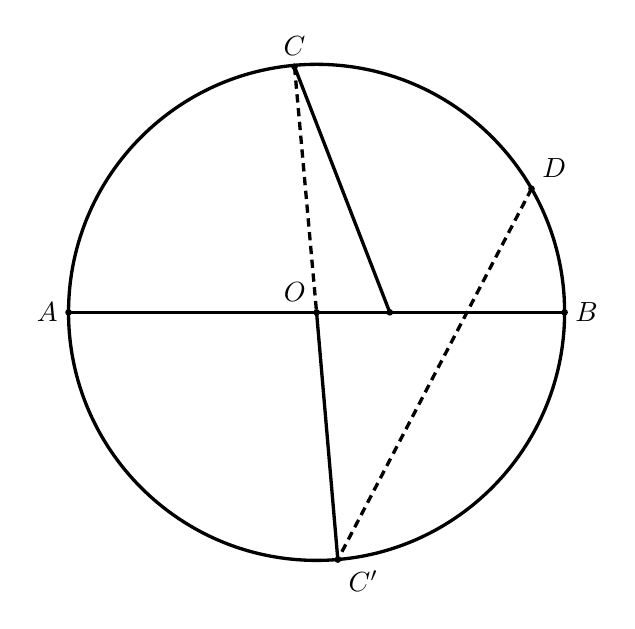
\begin{tikzpicture}[line width=1.2pt, line join=round]

% Named coordinates
\coordinate (O) at (0,0);
\coordinate (A) at (-3.15,0);
\coordinate (B) at (3.15,0);
\coordinate (C) at (-0.28,3.12);
\coordinate (Cp) at (0.27,-3.14);
\coordinate (D) at (2.73,1.57);
\coordinate (P) at (0.93,0);

% Circle centred at O, radius 3.15
\draw (O) circle (3.15);

% Solid segments
\draw (A) -- (B);
\draw (C) -- (P);
\draw (Cp) -- (O);

% Dashed segments
\draw[dash pattern=on 3pt off 2pt] (C) -- (O);
\draw[dash pattern=on 3pt off 2pt] (D) -- (Cp);

% Points
\foreach \p in {O,A,B,C,Cp,D,P} \fill (\p) circle (1.2pt);

% Labels
\node[above left] at (O) {$O$};
\node[left] at (A) {$A$};
\node[right] at (B) {$B$};
\node[above] at (C) {$C$};
\node[above right] at (D) {$D$};
\node[below right] at (Cp) {$C'$};

\end{tikzpicture}
\end{document}